\section{Homodyne detection scheme}\label{sec-homodyne}
{POVM of $m$ photon counts $\hat P_m$ for non-ideal detector of quantum efficiency $\eta$ is given by{~\cite{kelley1964theory}}},
\begin{equation}
    \hat{P}_m=:\frac{(\eta \hat{n})^me^{-\eta \hat{n}}}{m!}:, \label{eq:hpm}
\end{equation}
where $\hat{n}=\hat{a}^\dag\hat{a}$ is the number operator and $:\ :$ designates normal order. {We are ignoring dark counts, because including them is simply a shift of the dependency in the form $\hat{n}+\nu$}.  Since events of registation photon counts $m_1$ and $m_2$ are independent, POVM of the homodyne measurement scheme  (see Fig.~\ref{fig:homodyne}) is a product of POVMs given by Eq.{~\eqref{eq:hpm}} with appropriate indices (See e.g.{~\cite{vogel1993statistics}}),
\begin{equation}
    \hat{P}_{m_1,m_2}=\langle\hat{P}_{m_1,m_2}\rangle =
    :\prod_{l=1}^2\frac{(\eta_l\hat{n}_l)^{m_l}}{m_l!}
    e^{-\eta_l\hat{n}_l}
    :,
\end{equation}
{and the probability of detecting $m_1$ and $m_2$ photon counts is given by averaging this POVM,}
\begin{equation}
    P_{m_1,m_2}=\langle\hat{P}_{m_1,m_2}\rangle =\left\langle
    :\prod_{l=1}^2\frac{(\eta_l\hat{n}_l)^{m_l}}{m_l!}
    e^{-\eta_l\hat{n}_l}
    :
    \right\rangle.\label{eq:h-sred}
\end{equation}
{Hereinafter we will assume both signal and LO to be in coherent states to simplify our analysis, returning to the case of non-coherent signal later in this section.}

{To obtain transformed amplitudes we will use the unitary BS transform} 
\begin{equation}
    \hat{R}_\theta=\begin{pmatrix}
C&S\\-S&C
\end{pmatrix},
\end{equation}
{where we have introduced the following designations:}
\begin{align}
\begin{split}
    \cos\theta&\equiv C,\\
    \sin\theta&\equiv S.
\end{split}
\end{align}
{From the BS transform we may obtain the relations between input and output as follows:}
\begin{equation}
    \begin{pmatrix}
\hat{a}_1\\\hat{a}_2
\end{pmatrix}=
\hat{R}_\theta
\begin{pmatrix}
\hat{a}\\\hat{a}_L
\end{pmatrix}=
\begin{pmatrix}
C\hat{a}+S\hat{a}_L\\
-S\hat{a}+C\hat{a}_L
\end{pmatrix}, \label{eq:h-BS}
\end{equation}
{from which we obtain the transformed amplitutes as}
\begin{align}
\begin{split}
|\alpha_1|&=|C\alpha+S\alpha_L|, \\
|\alpha_2|&=|-S\alpha+C\alpha_L|.
\end{split} \label{eq:amplitudes}
\end{align}
Introducing the photon count difference 
\begin{equation}
    \delta m = m_1-m_2,
\end{equation}
we may express the statistical distribution of the photon count difference in a homodyne scheme, denoted $P$, as a product of two Poisson distributions, in the form
\begin{equation}
    P=\sum_{m_2}
\frac{(\eta_1|\alpha_1|^2)^{\delta m+m_2}}{(\delta m+m_2)!}e^{-\eta_1|\alpha_1|^2}
\frac{(\eta_2|\alpha_2|^2)^{m_2}}{m_2!}e^{-\eta_2|\alpha_2|^2}.
\label{eq:poisson}
\end{equation}
By performing the $m_2$ summation we may express $P$ as ~\cite{skellam1946frequency}
\begin{equation}
  P=e^{-\eta_1|\alpha_1|^2}e^{-\eta_2|\alpha_2|^2}
\left(\frac{\eta_1|\alpha_1|^2}{\eta_2|\alpha_2|^2}\right)^{\frac{\delta m}{2}}
I_{\delta m}\left(2\sqrt{\eta_1\eta_2|\alpha_1|^2|\alpha_2|^2}\right),\label{eq:accurate}
\end{equation}
where $I_k(z)$ is the modified Bessel function of the first kind. %\hl{While we may work with Eq.{~\eqref{eq:accurate}} and use Gaussian approximation of Bessel function (an older approach introduced in{~\cite{freyberger1993photon}}), our results suggest that it is better to use Gaussian approximation of the Poisson distribution, given by Eq.{~\eqref{eq:poisson}} due to POVMs' domain of definition. The first approach ("Bessel approximation") and the problem it causes explained further in Appendix{~\ref{app:bessel}}, and the second approach ("Gaussian approximation") is used in this section.}
\hl{Our findings reveal that the approach of approximating the Skellam distribution using the asymptotic expansion of the modified Bessel function of the first kind is not applicable for POVM construction in the asymmetrical case, which we discuss in Appendix{~\ref{app:bessel}}.}

It is straightforward to show that the Poisson distribution of a discrete variable $x$ with mean $\lambda$ can be approximated by the normal distribution of a continuous variable $x$ with both mean and variance equal to $\lambda$ when $\lambda \gg 1$. Applying this approximation to Eq.{~\eqref{eq:poisson}}, replacing the summation with integration, and using the LO approximation ($|\alpha_L|\gg|\alpha|$) by rewriting the relevant sum and difference as:
\begin{align}
\begin{split}
\eta_1|\alpha_1|^2+\eta_2|\alpha_2|^2&=\left[\eta_1S^2+\eta_2C^2\right]|\alpha_L|^2+\left[\eta_1-\eta_2\right]CS|\alpha_L|\langle\hat{x}_\phi\rangle+{\mathcal{O}}\left(\frac{1}{|\alpha_L|}\right),\\
-\eta_1|\alpha_1|^2+\eta_2|\alpha_2|^2&=\left[-\eta_1S^2+\eta_2C^2\right]|\alpha_L|^2+\left[\eta_1+\eta_2\right]CS|\alpha_L|\langle\hat{x}_\phi\rangle+{\mathcal{O}}\left(\frac{1}{|\alpha_L|}\right),
\end{split}
\label{eq:small-o}
\end{align}
where
\begin{equation}
    \langle\hat{x}_\phi\rangle={2\Re\alpha e^{-i\phi_L}}
\end{equation}
is the average of the phase-rotated quadrature operator of the signal
mode, defined as
\begin{equation}
\hat{x}_\phi=\hat{a}e^{i\phi}+\hat{a}^\dag e^{-i\phi},
    \label{eq:quad-op}
\end{equation}
we obtain the Gaussian approximation for Eq.~\eqref{eq:accurate}, denoted $P_G$,
\begin{multline}
    P_G=\frac{1}{\sqrt{2\pi(\eta_1S^2+\eta_2C^2)|\alpha_L|^2}}
    \exp \biggl[-\frac{1}{2}\frac{
\left[\left(\eta_1+\eta_2\right)CS\right]^2}
{\eta_1S^2+\eta_2C^2}
\times\\\times
{\left(\frac{\delta m}{(\eta_1+\eta_2)CS|\alpha_L|}-\frac{\eta_1S^2-\eta_2C^2}{\left(\eta_1+\eta_2\right)CS}|\alpha_L|-\langle\hat{x}_\phi\rangle\right)^2}\biggr],\label{eq:Pgood}
\end{multline}
which may be rewritten in the form
\begin{equation}
{P}_G(x)=\frac{1}{\sqrt{2\pi(\eta_1S^2+\eta_2C^2)|\alpha_L|^2}}
    \exp \biggl[-\frac{1}{2}D{\left(x-\langle\hat{x}_\phi\rangle\right)^2}\biggr],
    \label{eq:Pgood-w-def}
\end{equation}
where designations
\begin{align}
    \begin{split}
        D&\equiv\frac{
\left[\left(\eta_1+\eta_2\right)CS\right]^2}{\eta_1S^2+\eta_2C^2},\\x&\equiv\frac{\delta m}{(\eta_1+\eta_2)CS|\alpha_L|}-\frac{\eta_1S^2-\eta_2C^2}{\left(\eta_1+\eta_2\right)CS}|\alpha_L|.
    \end{split}
    \label{eq:defs-x-D}
\end{align}
have been used. 

We will now construct the POVM corresponding to the Gaussian approximation $P_G$. To do so, we first note that \eqref{eq:Pgood} is the average of the POVM over coherent states,
\begin{equation}
    P_G=\langle\alpha|\hat{P}_G|\alpha\rangle.
\end{equation}
Moreover, in case of ideal scheme, $P_G$ (denoted $P_0$ for $\eta_1=\eta_2=1$ and $\theta=\frac\pi4$),
\begin{equation}
    \label{eq:p-0}
    P_0\left(x\right)\equiv
    \frac{1}{\sqrt{2\pi|\alpha_L|^2}}
    \exp \left[-\frac{1}{2}{\left(\frac{\delta m}{|\alpha_L|}-\langle\hat{x}_\phi\rangle\right)^2}\right],
\end{equation}
coincides with the $Q$-function for phase-rotated quadrature operator with appropriate variable change and normalization constant $|\alpha_L|^{-1}$,
\begin{equation}
    |\langle \alpha|x , \phi \rangle |^2 = \frac{1}{\sqrt{2\pi}}\exp\left[-\frac{1}{2}\left(x  - \langle \hat{x}_\phi\rangle\right)^2\right], 
\end{equation}
where $|x,\phi\rangle$ is the eigenstate of the phase-rotated quadrature operator~\eqref{eq:quad-op}. This means that in the case of the ideal scheme, the POVM is a projector onto $|x,\phi\rangle$, with appropriate normalization constant:
\begin{equation}
    \hat{P}_G=\frac{1}{|\alpha_L|}|x,\phi\rangle\langle x,\phi|,
\end{equation}
which is known. For the asymmetrical case we may write $P_G$ as a convolution of $P_0$ and a normalized Gaussian function $G(x,\sigma)$
\begin{equation}
    P_G\sim\int\mathop{dx'}G(x-x';\sigma)P_0(x'), \label{eq:theform}
\end{equation}
\begin{equation}
G(x, \sigma_D) = \frac{1}{\sqrt{2\pi\sigma_D}}\exp\left[-\frac{1}{2}\frac{x^2}{\sigma_D}\right],
\end{equation}
with $\sigma_D$ to be determined. The proportionality sign present in Eq.~\eqref{eq:theform} is a consequence of integrating with respect to $x'$ but normalizing integrand with respect to $\delta m$ as per Eq.~\eqref{eq:norm}, meaning that normalization constant is the linear factor relating definition of $x$ through $\delta m$. From Eq.~\eqref{eq:Pgood-w-def} we determine the proportionality constant to be $\left[\left(\eta_1+\eta_2\right)CS|\alpha_L|\right]^{-1}$, ensuring that the set of POVM would sum up to identity. This allows us to write the desired POVM as follows:
\begin{equation}
\hat{P}_G= \frac{1}{\left(\eta_1+\eta_2\right)CS|\alpha_L|}\int\mathop{d^2x'}G(x-x',\sigma_D)|x',\phi\rangle\langle x',\phi|.
\label{eq:method-1}
\end{equation}

Since the convolution of two Gaussian functions results in another Gaussian function with its variance being the sum of the variances of the original functions,
\begin{equation}
    \int\mathop{dx'}e^{-\frac{(x-x')^2}{\sigma_D}}e^{-\frac{x{'}^{2}}{\sigma_0}}=\sqrt{\frac{\pi}{\frac{1}{\sigma_D}+\frac{1}{\sigma_0}}}\exp\left[-\frac{x^2}{\sigma_D+\sigma_0}\right],
    \label{eq:conv}
\end{equation}
if we set $\sigma_0=2$ (variance of Gaussian in Eq.~\eqref{eq:p-0}) and
\begin{equation}
     \sigma_D=\frac{2}{D}-2,\label{eq:h-G}
\end{equation}
and substitute these into Eq.~\eqref{eq:conv}, the resulting variance will be $\frac{2}{D}$, as per Eq.~\eqref{eq:Pgood-w-def}. 
{Definition given by Eq.{~\eqref{eq:h-G}} implies that $D\leq1$, so that $\sigma_D\geq0$. It is not difficult to see that this is always satisfied:}
\begin{equation}
    {\max D=\frac{\left(\eta_1+\eta_2\right)^2}{\left(\sqrt{\eta_1}+\sqrt{\eta_2}\right)^2}\leq1.}
\end{equation}
 Therefore, $D\leq1$ for all $\eta_1$, $\eta_2$, and $\theta$, as opposed to the situation described in Appendix{~\ref{app:bessel}}.

We obtain the desired POVM for the Gaussian approximation as:
\begin{equation}
\hat{{P}}_G=\frac{1}{(\eta_1+\eta_2)CS|\alpha_L|}\int \mathop{dx'} G(x-x'; \sigma_D)|x',\phi\rangle\langle x',\phi|,
\label{eq:homodyne-povm}
\end{equation}
Note that 
\begin{equation}
    \lim_{D\to1}G(x,\sigma_D)=\delta(x),
\end{equation}
where $\delta(x)$ is the Dirac $\delta$-function, which is the expected behavior for Eq.~\eqref{eq:theform} to hold in the limiting case of an ideal scheme. Therefore, the constructed POVM is well-defined for all possible parameters of the homodyne scheme.

The ability of the homodyne scheme to reconstruct the quadrature of the state is well known, which is showcased by Eq.~\eqref{eq:homodyne-povm}.

It is worthwhile to assess how accurate $P_G$ is. To do so, the $L^1$ measure is defined as
\begin{equation}
    \mathtt{D}\left(P,{P}_{G}\right)\equiv
    \frac{1}{2}{\sum_{\delta m}
    \left|P -{P}_G\right|}.
\end{equation}

To illustrate the parameter dependency of the exact and approximate statistical distribution, we numerically calculate them using Eq.~\eqref{eq:accurate} and Eq.~\eqref{eq:Pgood}. The resulting distributions are presented in Fig.~\ref{fig:PLACEHOLDER}. For symmetrical variation of parameters $\eta_1$ and $\eta_2$, distributions and distance between distributions $\mathtt{D}$ changes asymmetrically, which is caused by sign change in Eq.~\eqref{eq:amplitudes}. For $\alpha=0$ symmetrical variation of $\eta_1$ and $\eta_2$ yields statistical distributions, both exact and approximate, as mirror-images of each other, with equal $\mathtt{D}$, as expected. Further calculations reveal that global minima of $\mathtt{D}$ coincide with parameters that shift the global maxima of statistical distributions to be at $0$.

A study of the dependence on amplitude parameters is shown in Fig.~\ref{fig:amplitude}. Both curves behave as expected: monotonic increase for increasing $|\alpha|$ with fixed $|\alpha_L|$ and monotonic decrease for increasing $|\alpha_L|$ with fixed $|\alpha|$. \hl{However, note that for the LO amplitude deviation it becomes significant that the function {\eqref{eq:Pgood}} is normalized in the sense of}
\begin{equation}
    {\sum_{\delta m}
    P_G
    %(x)
    =1,}
    \label{eq:norm}
\end{equation}
\hl{since the normalization constant of the function is dependent on $|\alpha_L|$. Rigorously, re-normalizing the function to $1$ is always needed due to us dealing with finite amplitude of LO, therefore we will always re-normalize the distribution numerically.}
In Fig.~\ref{fig:amplitude}b we may see that approximation is still adequate even when re-normalization of $P_G$ to $1$ is needed. Local maxima and minimas are present as well. \hl{Adequence of Gaussian approximation with numerical re-normalization is an oddity of weak signal amplitude $|\alpha|\ll\left[2(\eta_1S^2+\eta_2C^2)\right]^{-\frac{1}{2}}$.}
%This is caused by significance of discritization  for these parameters,  Degeneration is also causing the presented local minima. This behaviour is presented only for weak signals so that $|\alpha|<\sqrt{(\eta_1S^2+\eta_2C^2)}$, otherwise distance between numerically normalized distribution and exact distribution is greater than for normalized.

We may also plot the distance between distributions as a function of deviation from the ideal scheme, defined by the relation
\begin{equation}
        \delta\theta\equiv\frac{\pi}{4}-\theta,
\end{equation}
or as a function of $\eta_1$ ($\eta_2$) with fixed $\eta_2$ ($\eta_1$). The results are presented in Fig.~\ref{fig:delta-theta} and Fig.~\ref{fig:delta-eta}. We can see that the global minima of these functions depend on $\delta\theta$ as well as $\eta_1$ and $\eta_2$, shifting from zero for asymmetrical parameters. We may once again see that minimal distance between statistical distributions for non-ideal parameters corresponds to shifting global maxima of statistical distributions to be at $0$ -- this is seen by curves having global minima not at $\delta\theta=0$ and $\eta_{1}=1$ or $\eta_{2}=1$ respectively. 
We may also see the agreement at critical points $\pm\frac{\pi}{4}$ seen at Fig.~\ref{fig:delta-theta}. \hl{This is expected behaviour. While rigorously we cannot apply strong LO approximation for these critical points, since the condition $\eta_1|\alpha_1|^2\gg1$  (or $\eta_2|\alpha_2|^2\gg1$ ) does not hold in these cases, at these points one of the transformed amplitudes detected is proportional to only $|\alpha_L|$ and the other only to $|\alpha|$ (See Eq.{~\eqref{eq:amplitudes})}. Since $|\alpha_L|\gg|\alpha|$, if efficiencies of the detector arms detecting $\sim|\alpha_L|$ amplitude are equal, both exact and approximate distributions are rendered essentially the same, resulting in the same distance between them. Which is why, for example, the blue curve in Fig.{~\ref{fig:delta-theta}}, plotted for  $\eta_1=1, \eta_2=0.5$ agrees with the black curve, plotted for the relevant parameter $\eta_1=1$, at point $\delta\theta=-\frac{\pi}{4}$ -- transformed amplitudes are given by $\eta_1|\alpha_L|$ and $\eta_2|\alpha|$, and $\eta_1$ are equal for them. Likewise, the blue curve agrees with the green curve, plotted for the relevant parameter $\eta_2-0.5$, at point $\delta\theta=\frac{\pi}{4}$, correspoinding to the detector with efficiency $\eta_2$. The same logic applies to the orange curve.}
Monotonically increasing curves seen in Fig.~\ref{fig:delta-eta} correspond to the shifting of global maxima of statistical distributions to be further from $0$. Asymmetry between curves for symmetrical parameter change is again explained by sign change in Eq.~\eqref{eq:amplitudes}. 

\begin{figure}
    \centering
     \begin{minipage}[c]{.45\linewidth}
 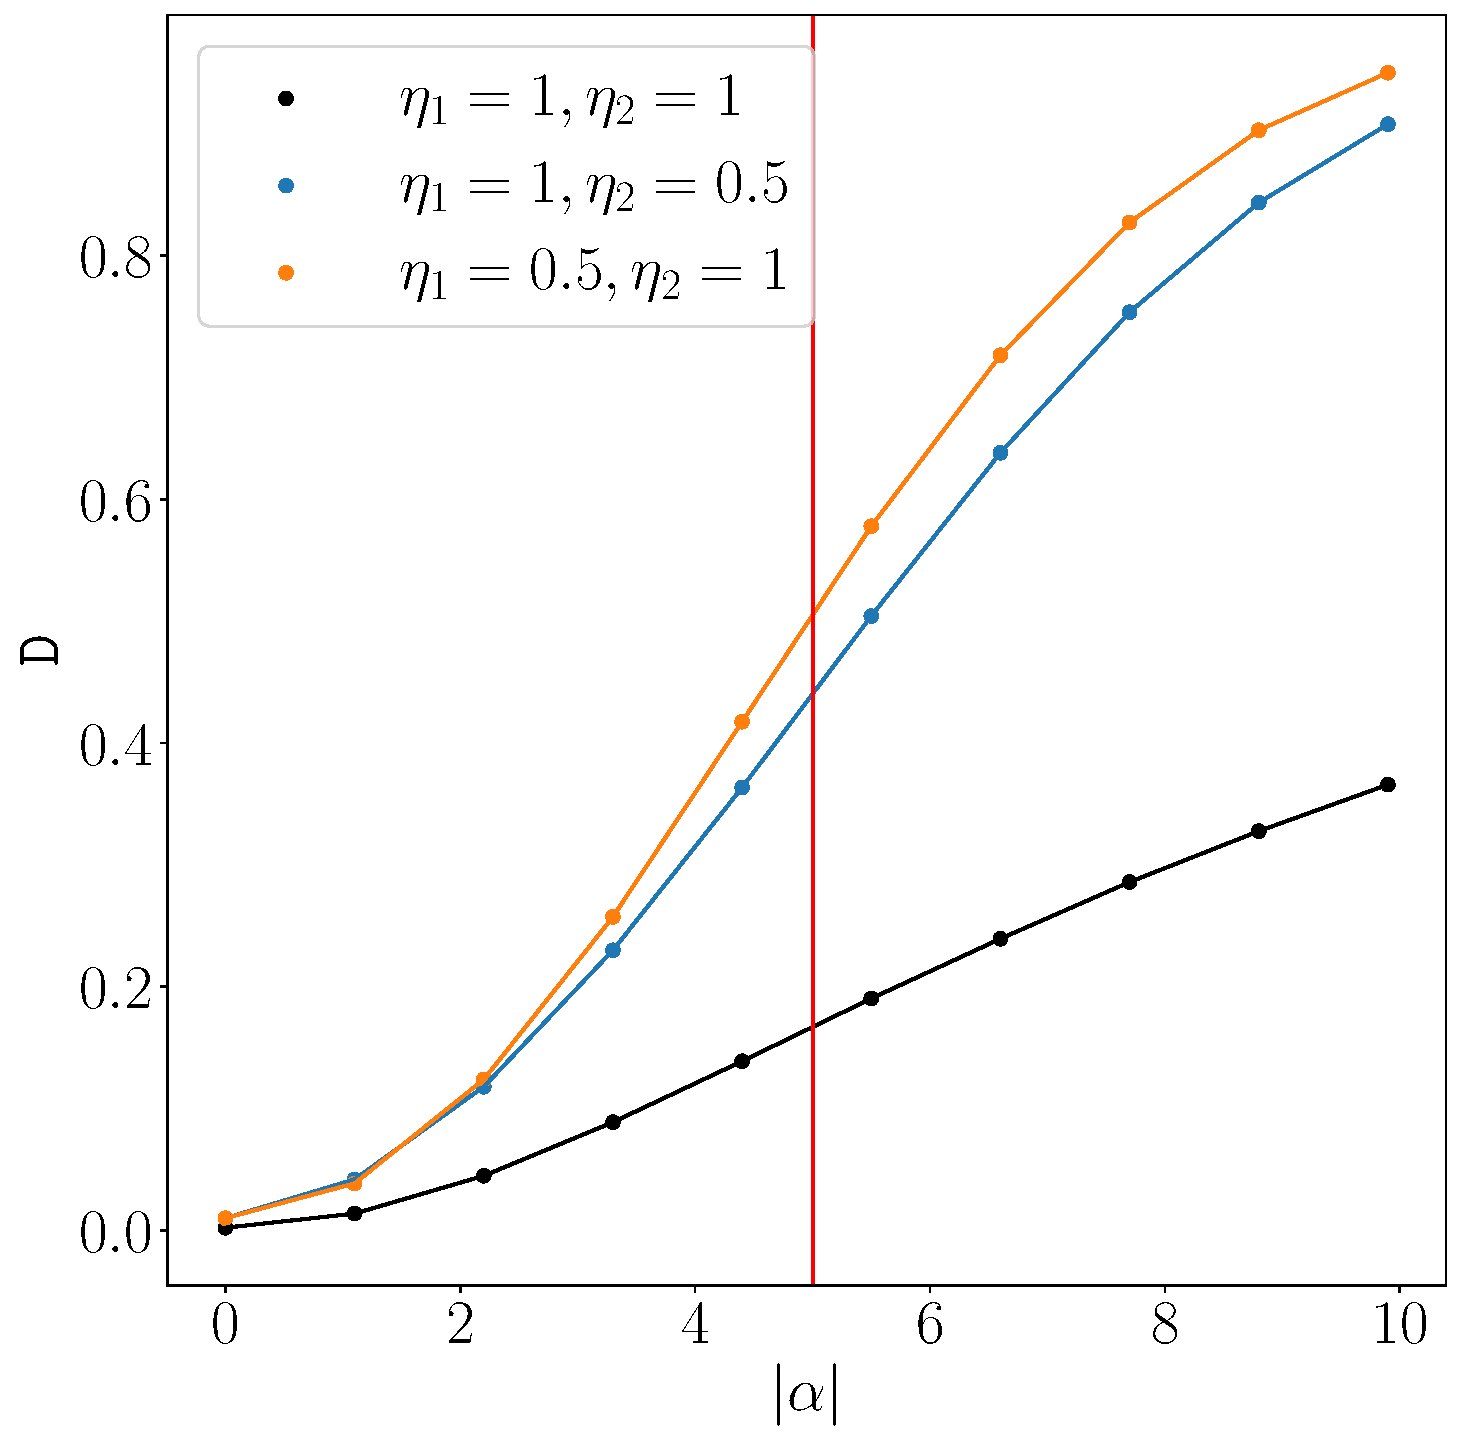
\includegraphics[width=\linewidth]{pics/homodyne/ED = ED(a)_5eta.pdf}
\subcaption[]{$|\alpha_L|=5$}
\end{minipage}
\hfill
\begin{minipage}[c]{.45\linewidth}
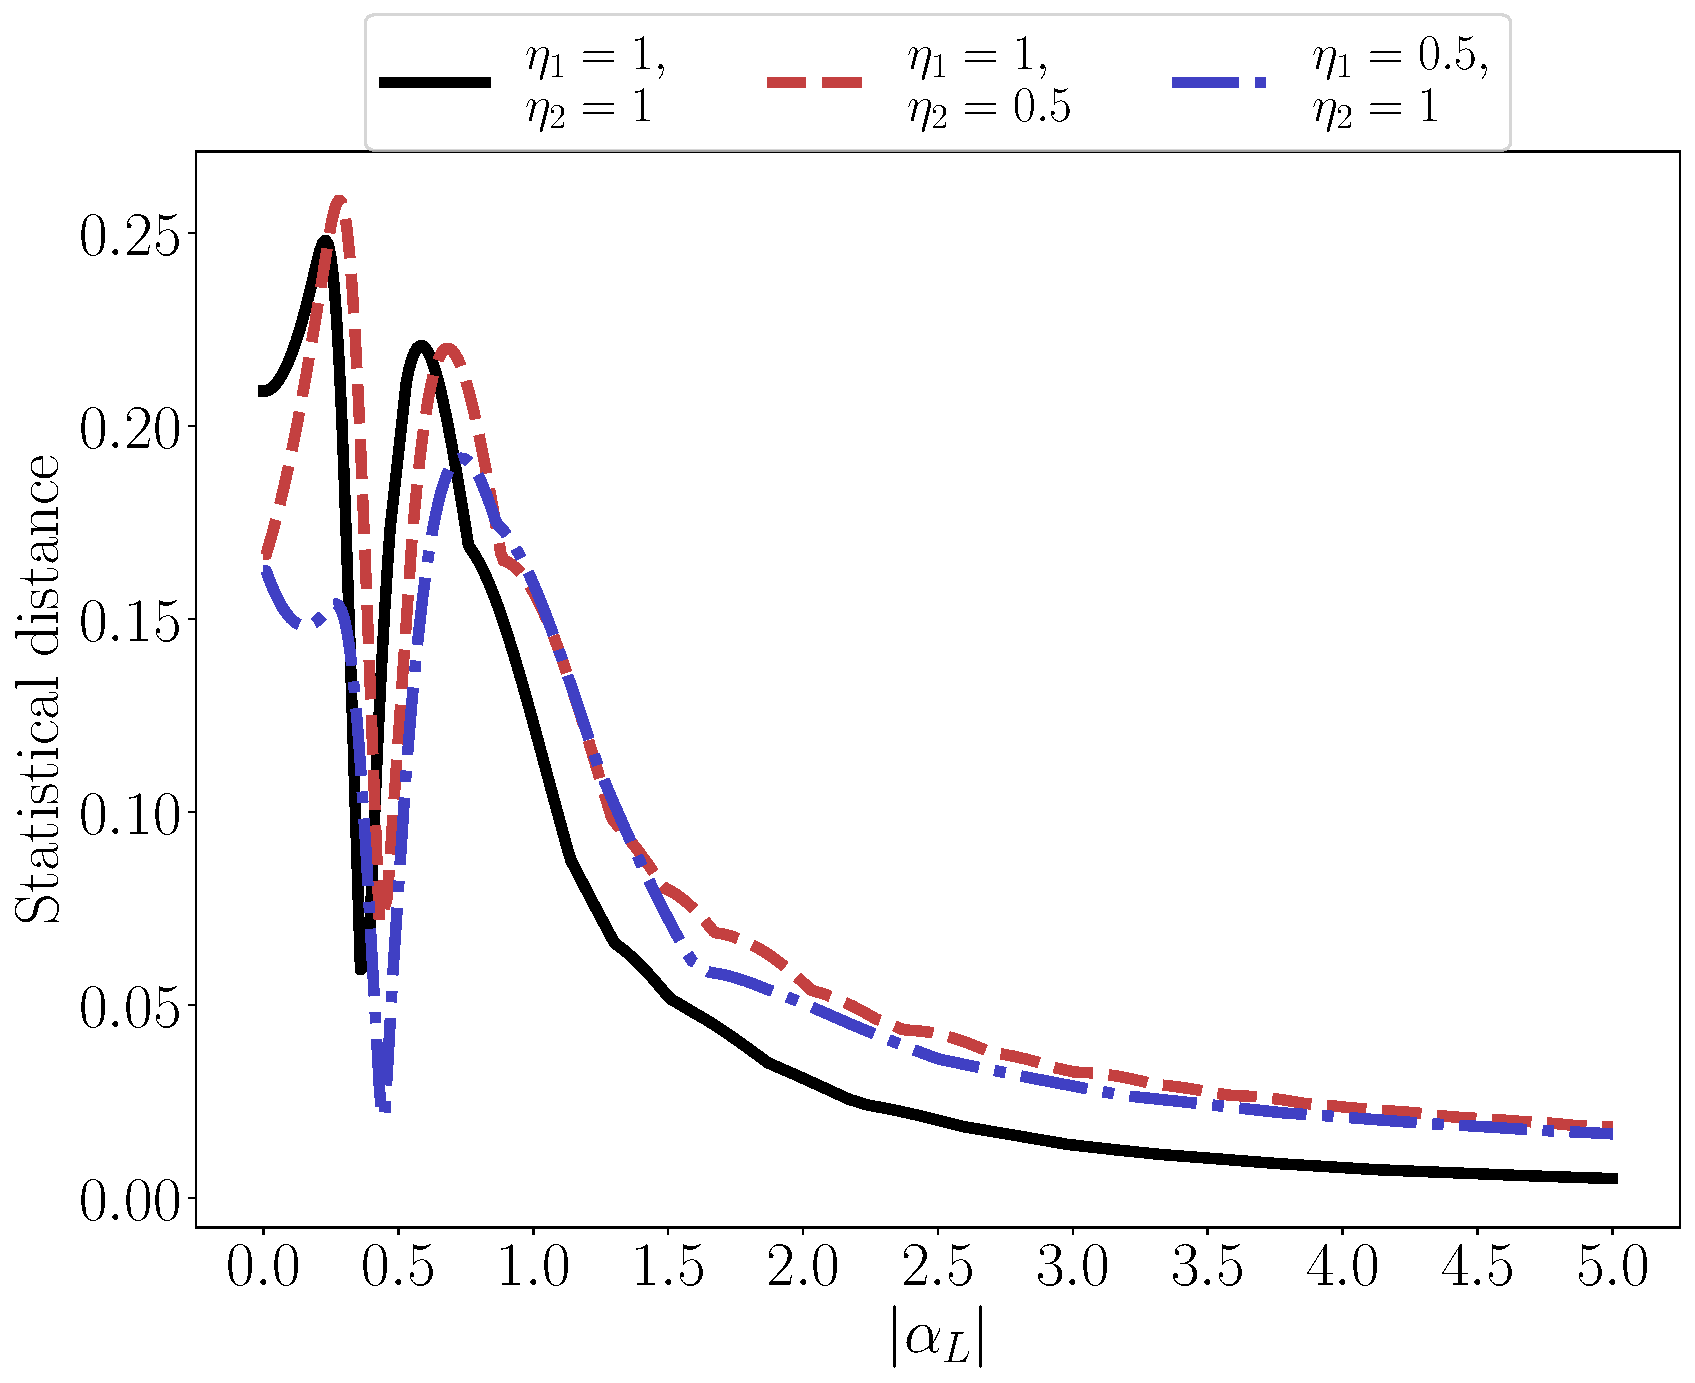
\includegraphics[width=\linewidth]{pics/homodyne/ED = ED(al).pdf}
\subcaption[]{$|\alpha|=0.1$}
        \end{minipage}
    \caption{
    Numerically calculated distance between the exact distribution and the Gaussian approximation as a function of (a) signal amplitude and (b) LO amplitude for different parameters of the beam splitter and detector efficiencies in the asymmetrical homodyne scheme. Red vertical line signifies $|\alpha|=|\alpha_L|$. \hl{More points are added when we expect anomalous behaviour.}
    }\label{fig:amplitude}
\end{figure}

\begin{figure}
    \centering
    \begin{minipage}[c]{.45\linewidth}
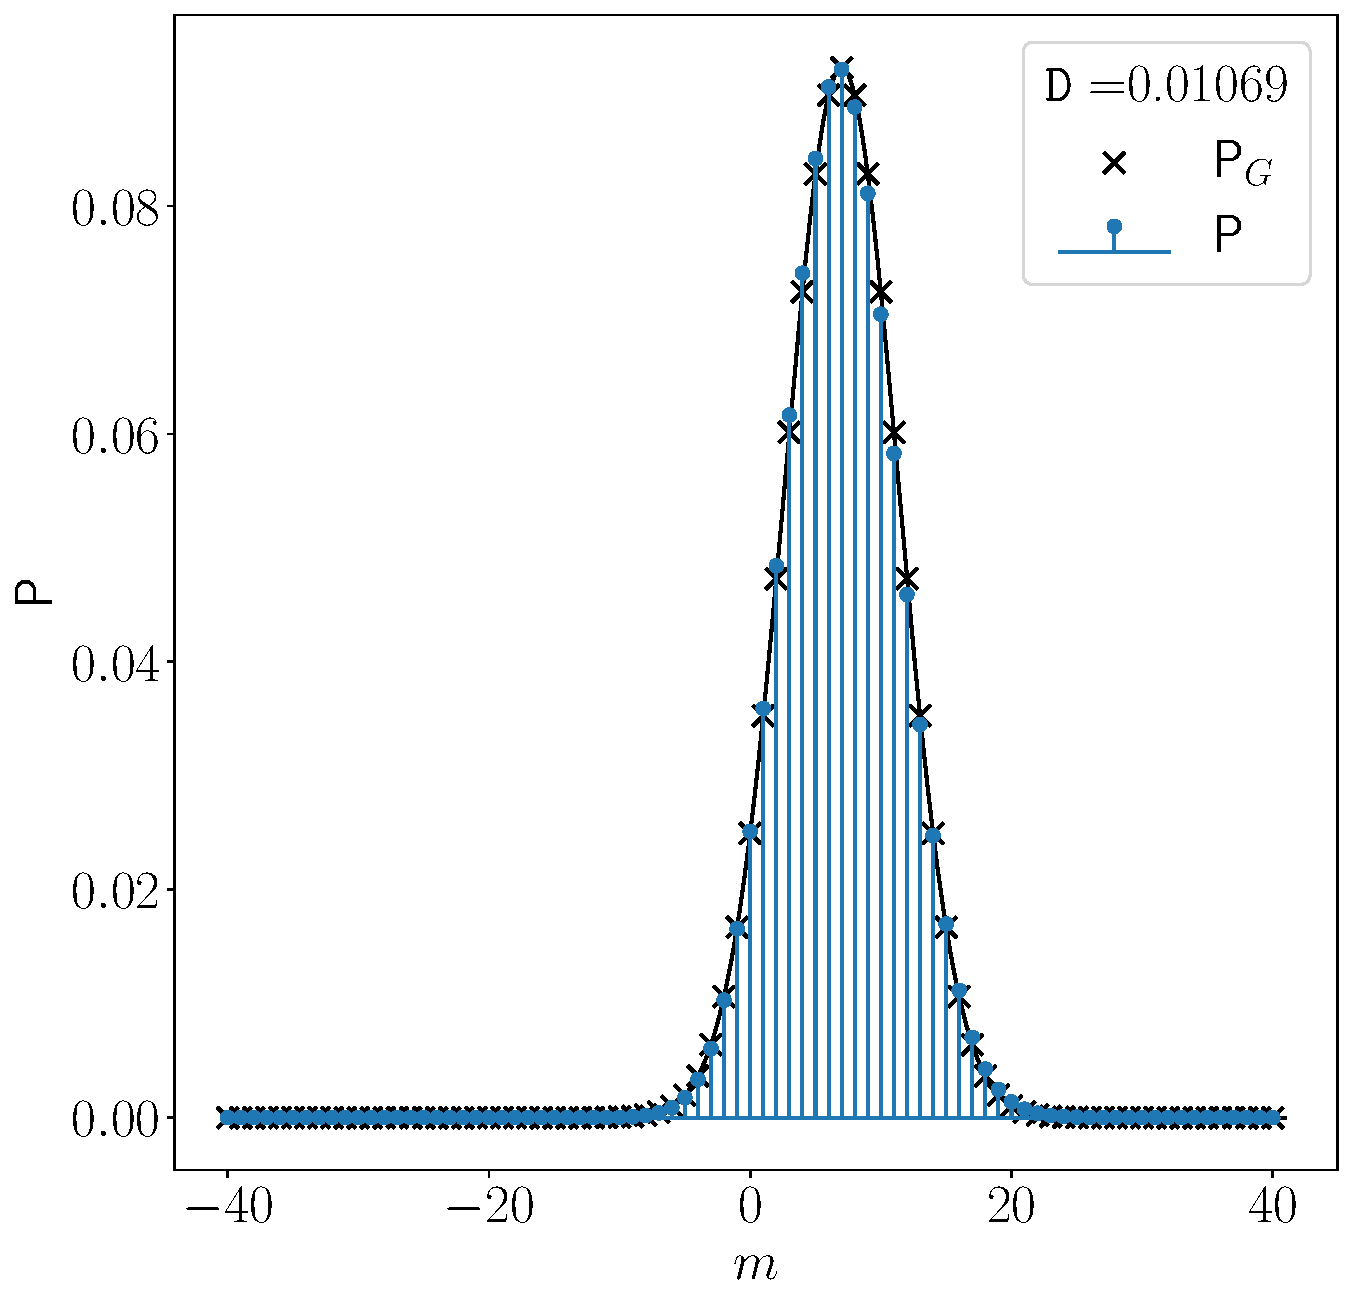
\includegraphics[width=\linewidth]{pics/homodyne/eta1=1, eta2=0.5, theta=1.0.pdf}
\subcaption[]{$\eta_1=1,\eta_2=0.5$}
        \end{minipage}
\hfill
        \begin{minipage}[c]{.45\linewidth}
 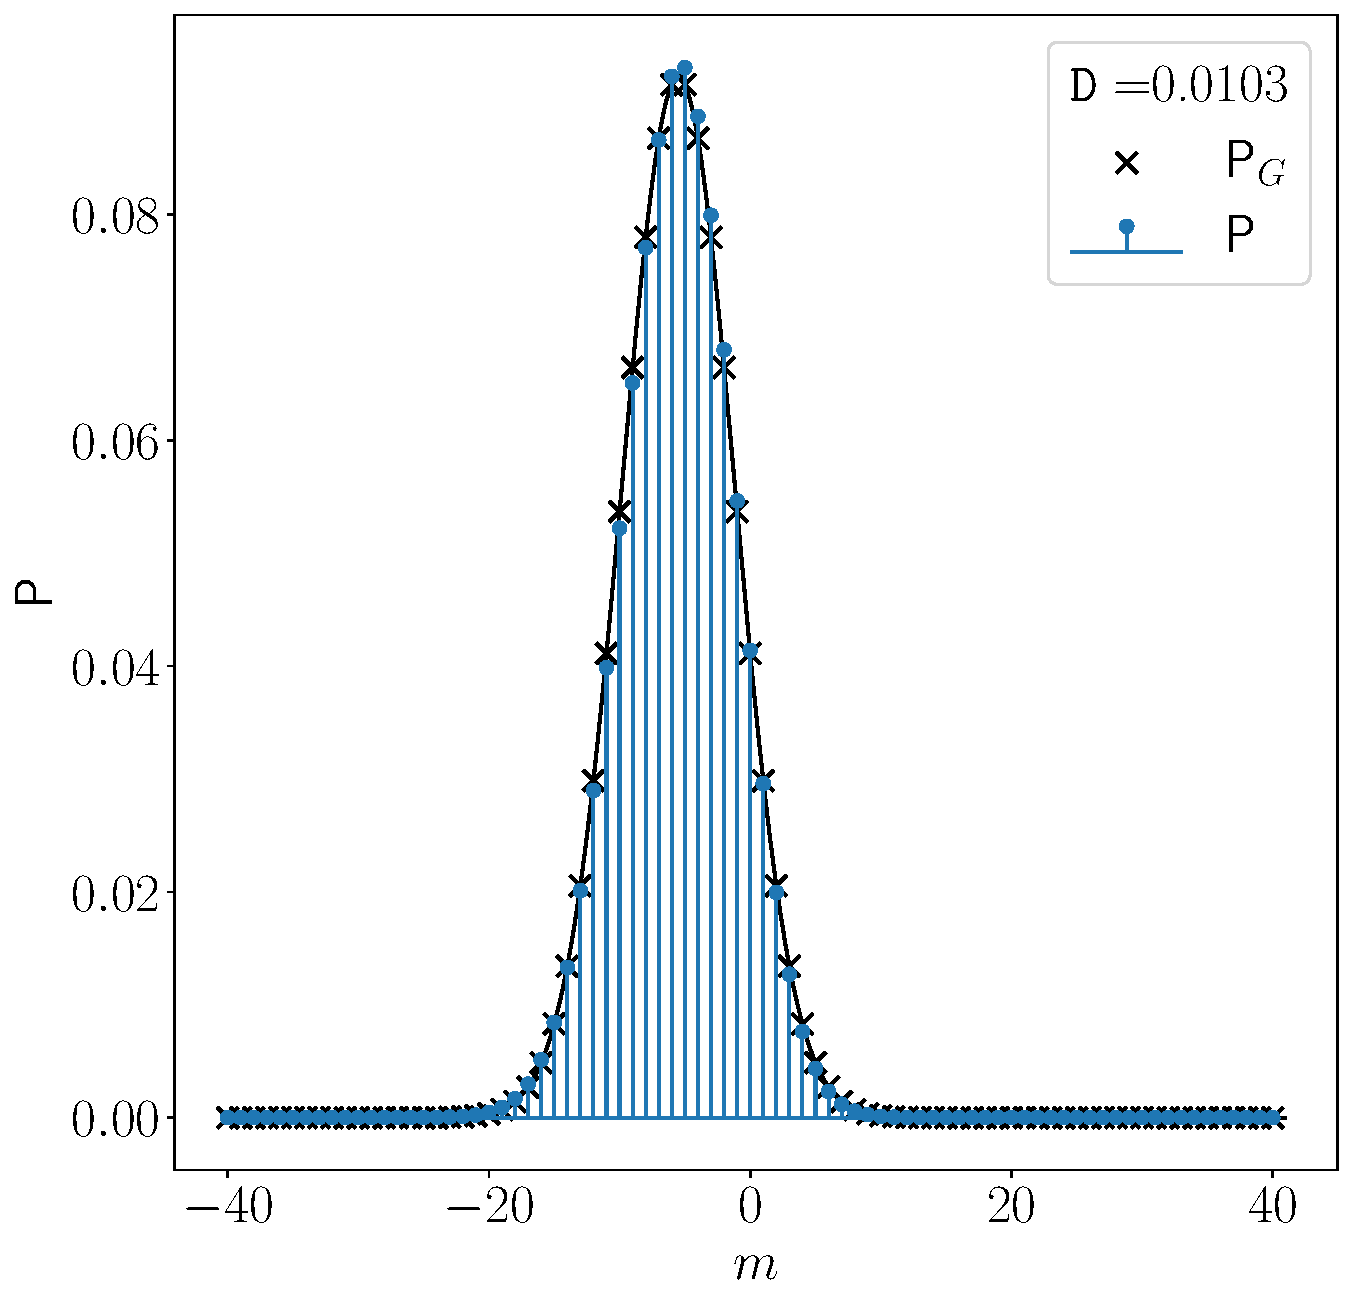
\includegraphics[width=\linewidth]{pics/homodyne/eta1=0.5, eta2=1, theta=1.0.pdf}
\subcaption[]{$\eta_1=0.5,\eta_2=1$}
\end{minipage}
    \caption{
    Numerically calculated statistical distributions of photon count difference in the asymmetrical homodyne scheme, given by  Eq.~\eqref{eq:accurate} (blue) and Eq.~\eqref{eq:Pgood} (black) for different parameters of quantum efficiencies, with $|\alpha|=0.1$ and $|\alpha_L|=5$. Shifting of global maxima for approximation is explained by the term proportional to $|\alpha_L|$ in Eq.~\eqref{eq:Pgood}, and for exact formulae by the terms proportional to $|\alpha_L|$ in Eq.~\eqref{eq:accurate}, which is better seen as the argument of the modified Bessel function in Eq.~\eqref{eq:Skellam}. Asymmetry in distributions with symmetrical parameter variation is explained by dependence on $|\alpha|$. Note the significant difference in $\mathtt{D}$.
    }\label{fig:PLACEHOLDER}
\end{figure}

\begin{figure}
    \centering
    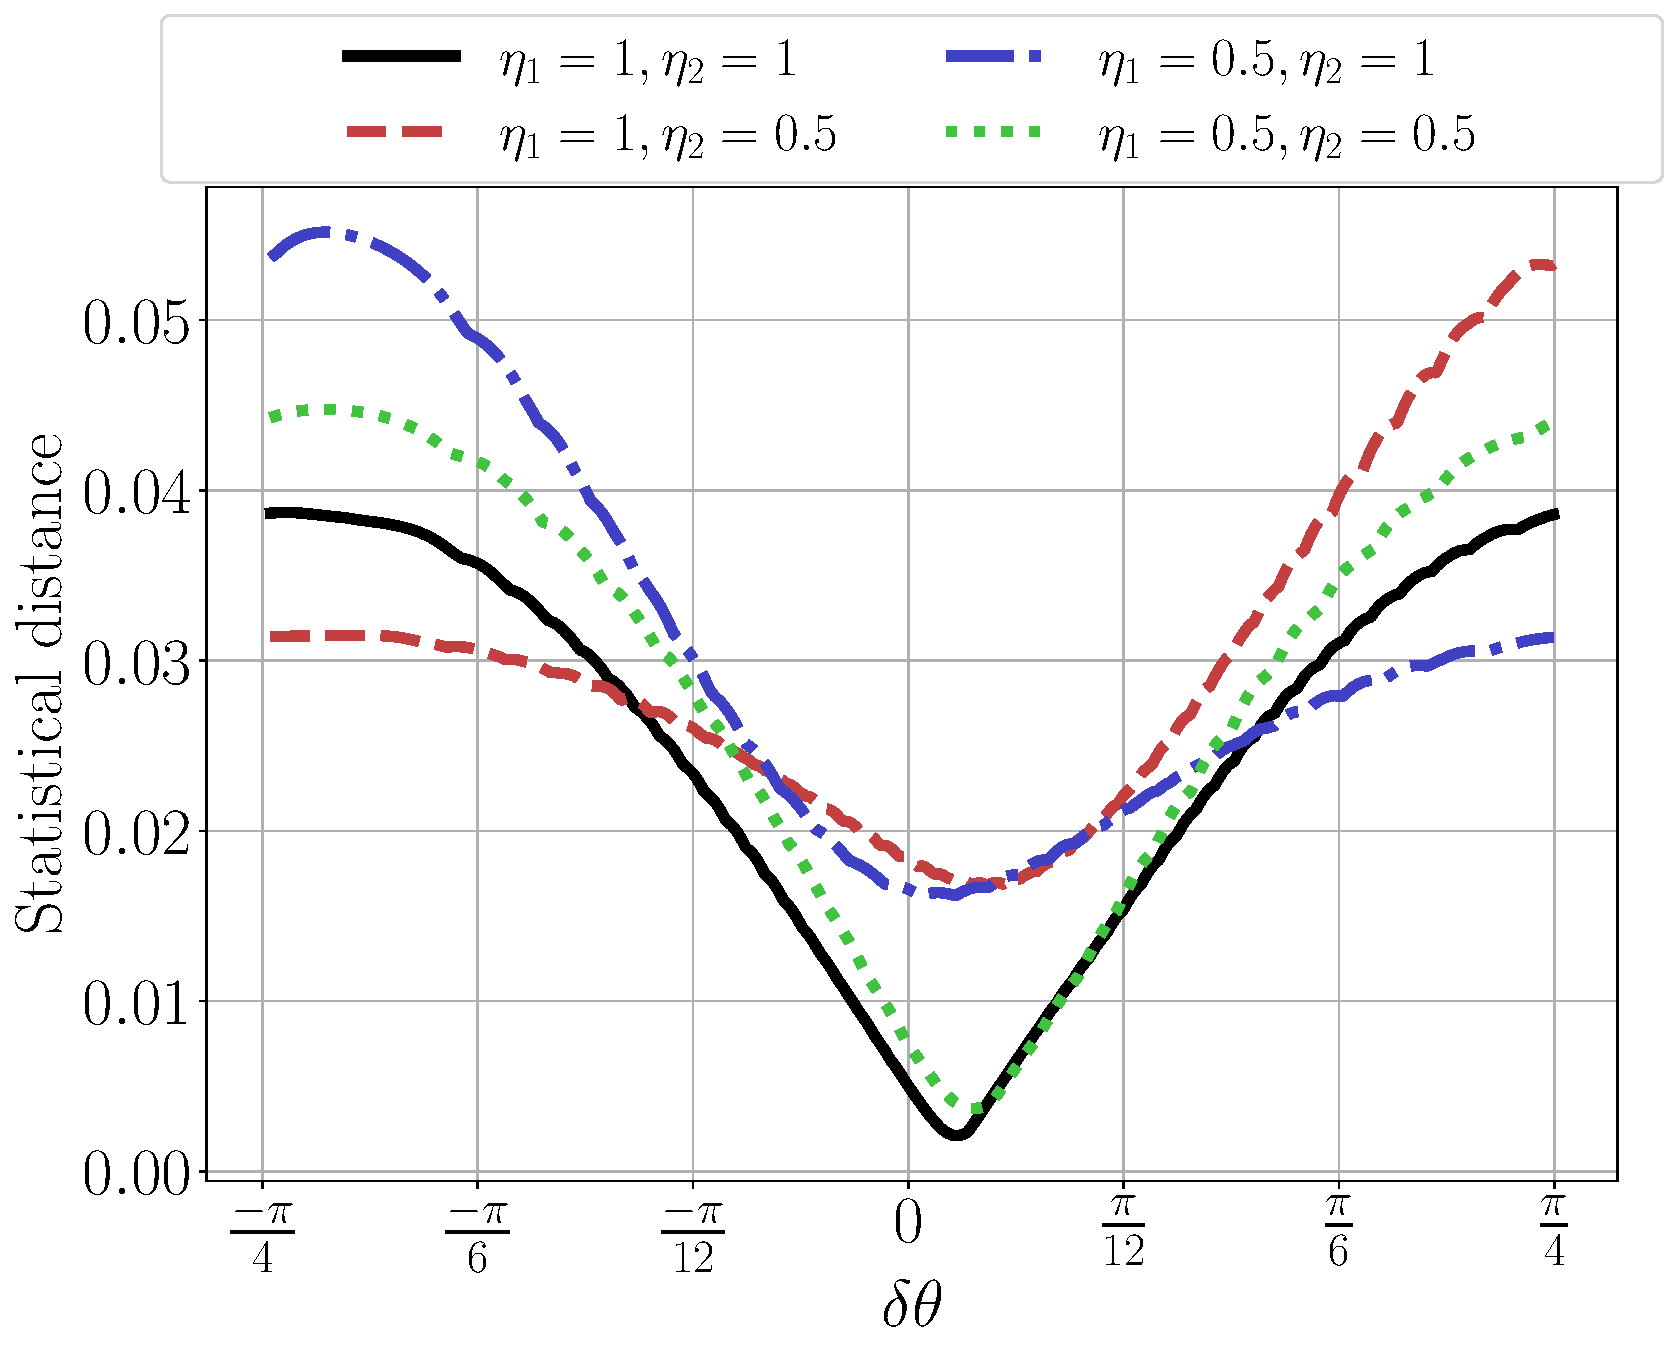
\includegraphics[width=0.75\linewidth]{pics/homodyne/full.pdf}
    \caption{Numerically calculated distance between the exact distribution of photon count difference in the asymmetrical homodyne scheme and its Gaussian approximation as a function of deviation from a balanced beam splitter for different detector efficiencies, with $|\alpha|=0.1$ and $|\alpha_L|=5$. Shifting of global minima $\mathtt{D}$ coincides with parameters that shift the global maxima of statistical distributions to be at $0$.}% Note the agreement at critical points $\pm\frac{\pi}{4}$ \hl{between some of the curves} -- \hl{this is caused by full reflection (transmission) into one output port of the scheme, which makes statistical distributions at these points essentially the same for equal relevant efficiency parameters}.}
    \label{fig:delta-theta}
\end{figure}

\begin{figure}
    \centering
    \begin{minipage}[c]{.45\linewidth}
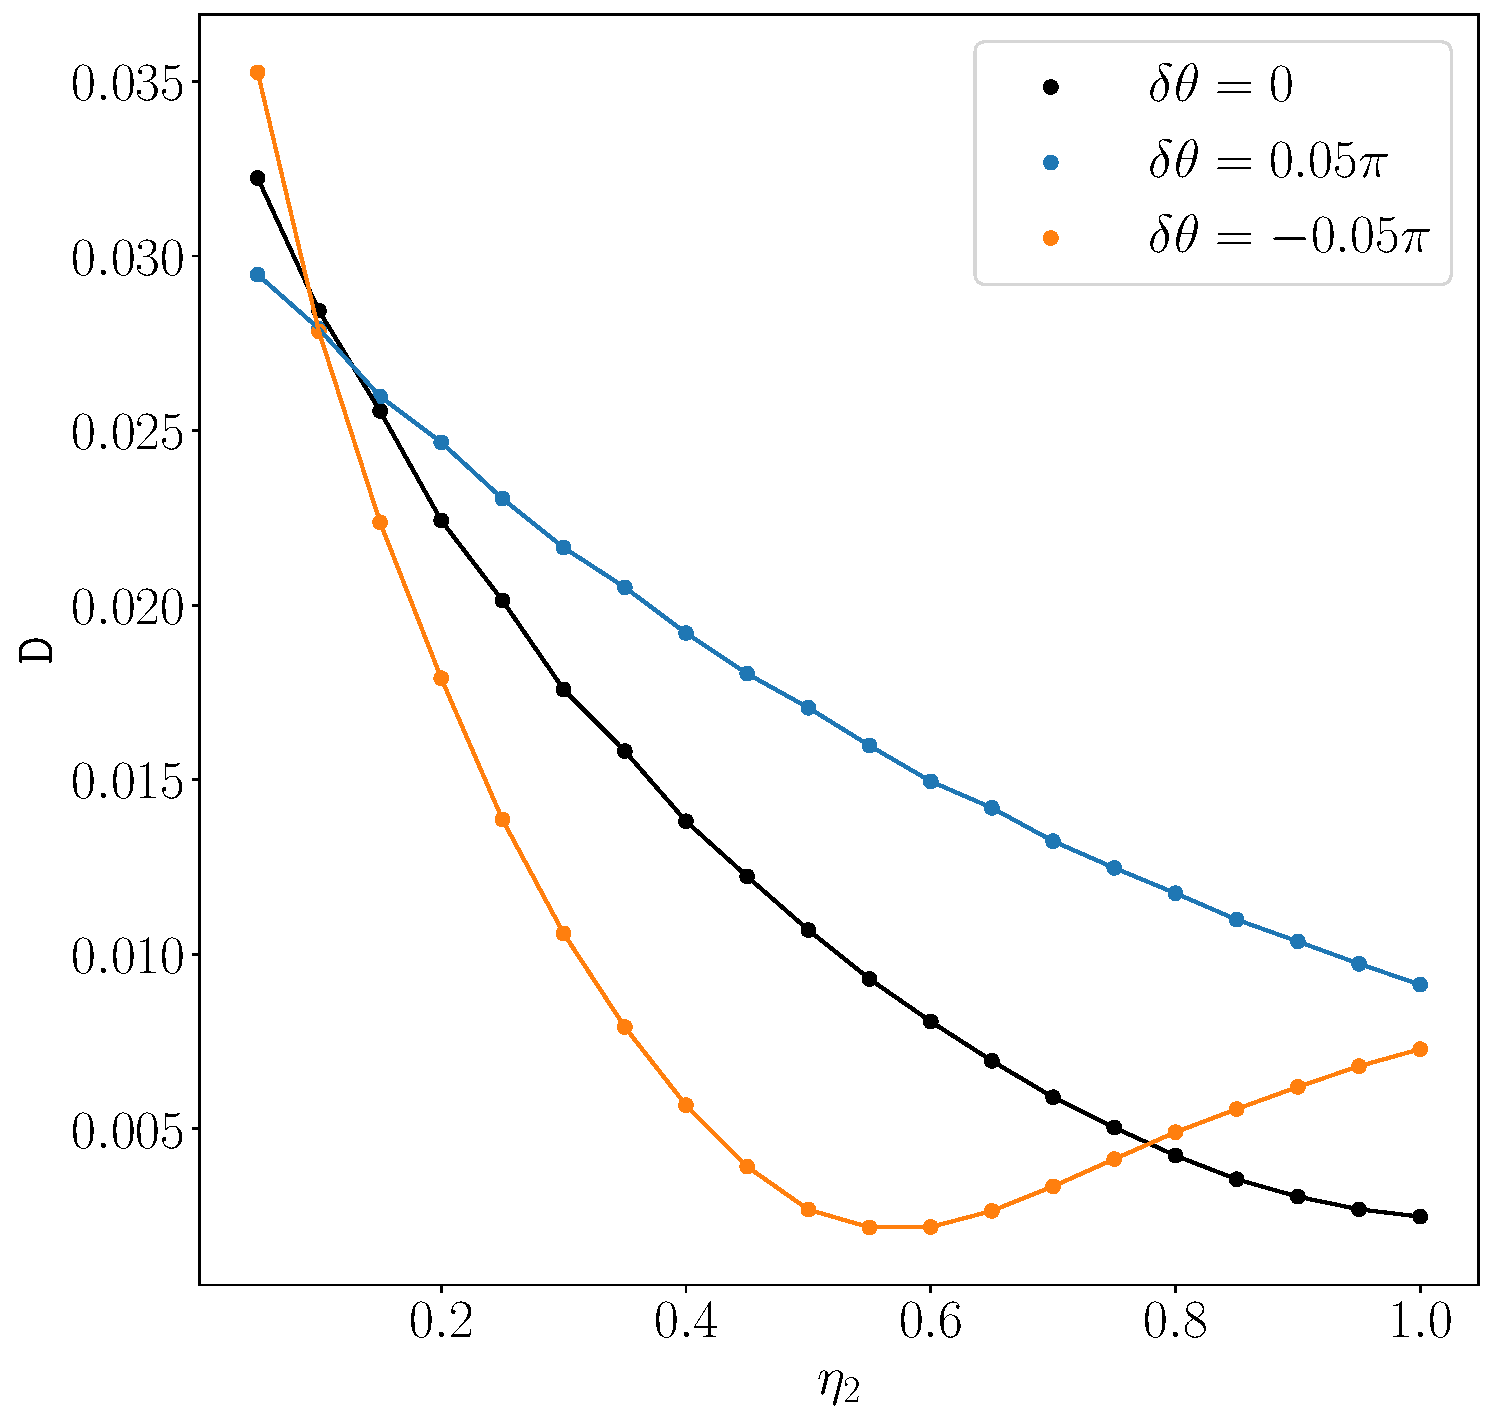
\includegraphics[width=\linewidth]{pics/homodyne/full1.pdf}
\subcaption[]{$\eta_1=1$}
        \end{minipage}
\hfill
        \begin{minipage}[c]{.45\linewidth}
 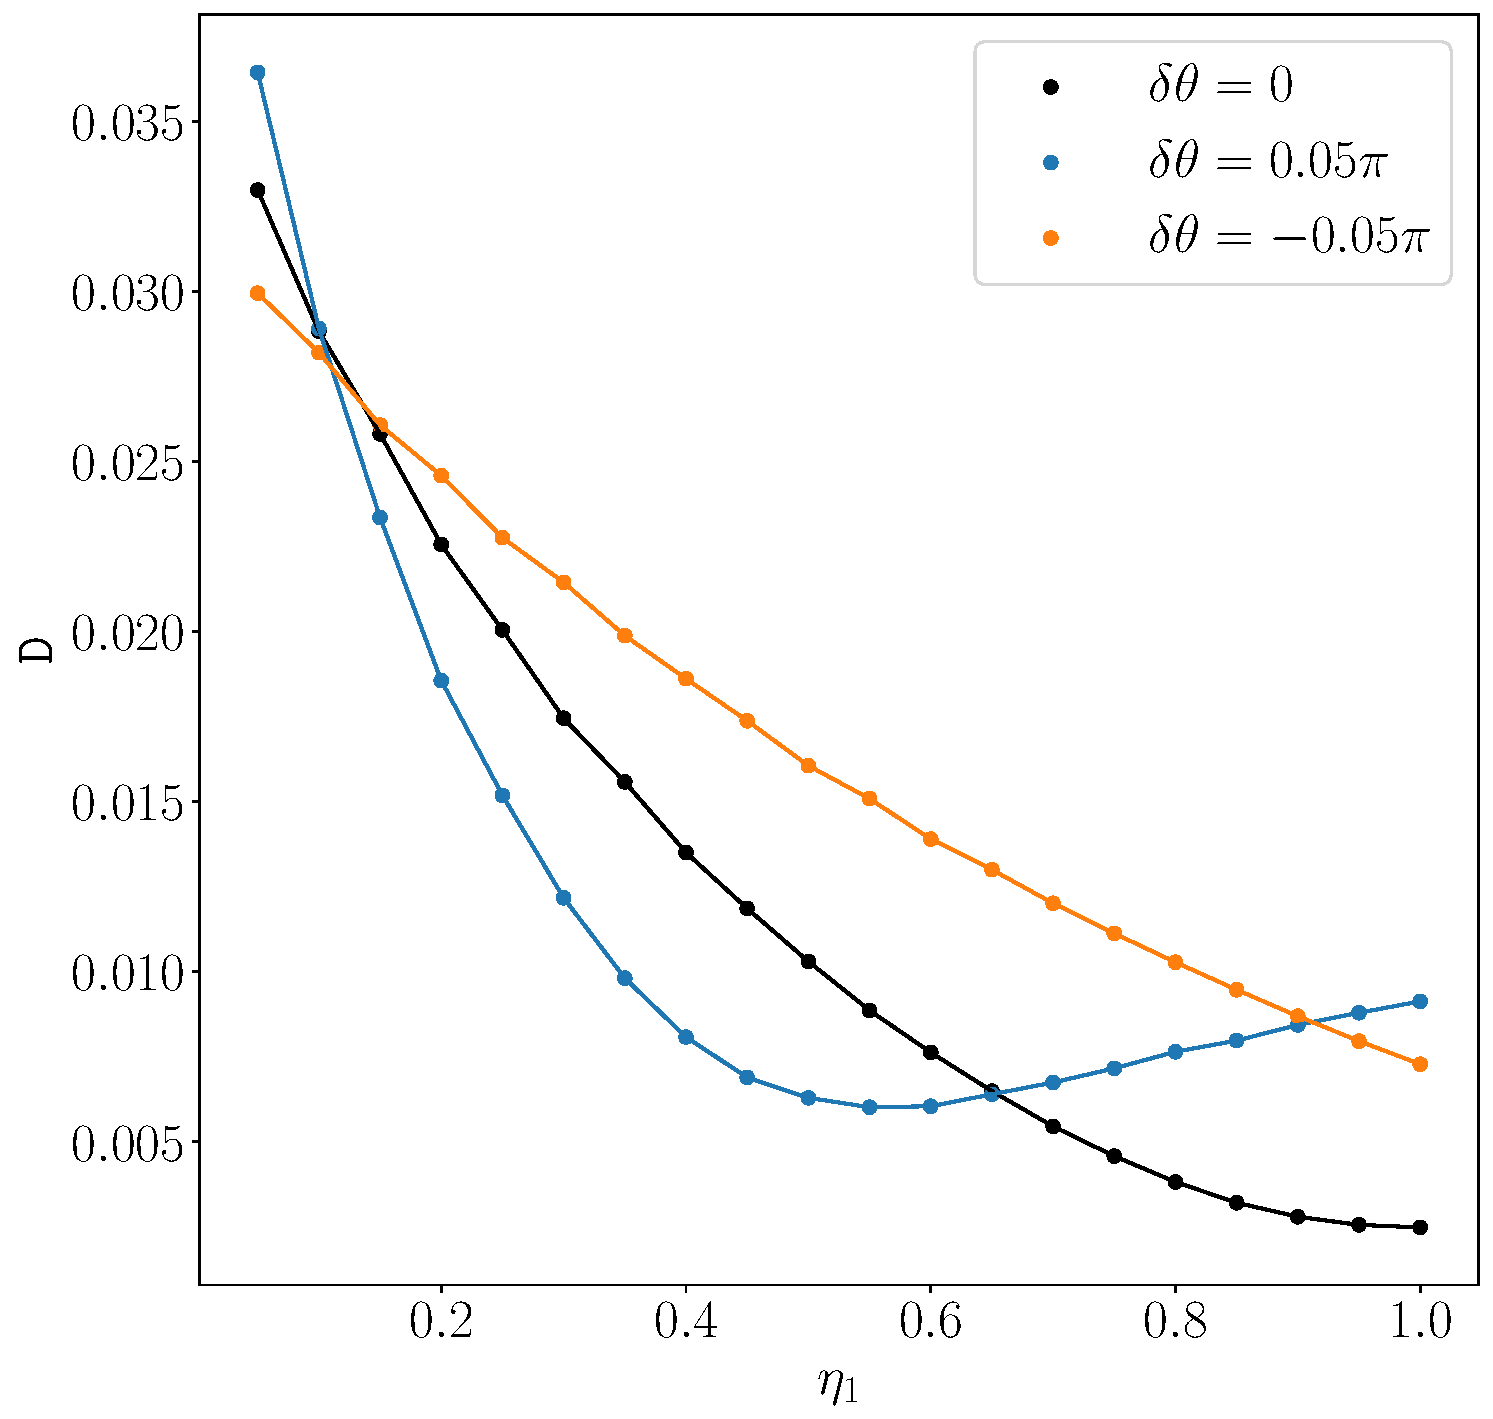
\includegraphics[width=\linewidth]{pics/homodyne/full2.pdf}
\subcaption[]{$\eta_2=1$}
\end{minipage}
    \caption{
    The numerically calculated distance between the exact distribution of photon count difference in the asymmetrical homodyne scheme and its Gaussian approximation as a function of deviation from equal detector efficiencies for different beam splitter parameters, with $|\alpha|=0.1$ and $|\alpha_L|=5$. For curves with global minima not at $\eta_1=1$ or $\eta_2=1$, parameters of both $\eta_1$ and $\eta_2$ coincide with parameters which shift the global maxima of statistical distributions to be at zero.
    }\label{fig:delta-eta}
\end{figure}

A similar methodology may be performed for a non-coherent signal state. To do so, both $P$ and $P_G$ need to be averaged with relevant $P$-function $P_\psi$, yielding relevant distributions $P^\psi$ and $P_G^\psi$,
\begin{equation}
P^\psi=\int \mathop{d^2\alpha} P_{\psi}(\alpha)P(\alpha).
\end{equation}

Here we present the results for the Fock state with $n=1$. Its $P$-function has the form \cite{vogel2006quantum}
\begin{equation}
    P_{(n)}(\alpha)=
    \sum_{k=0}^n \binom{n}{k}\frac{1}{k!} \partial_{\alpha}^k\partial^k_{\alpha^*}\delta(\alpha).
\end{equation}
The dependency of the distance between exact and approximate distributions on the efficiency of the detectors is very much like one for the coherent state and is therefore not presented. Results for dependency on $\delta\theta$ are presented in Fig.~\ref{fig:fock}. We may observe the global minima as always at $0$, and local minima at critical points. 
Global maxima are dependent on parameters of efficiency, and symmetrical parameter variation results in symmetrical distributions. \hl{Moreover, the same agreement at critical points between some of the curves as presented at Fig.{~\ref{fig:delta-theta}} can be seen -- this effect has the same explanation.} 
\begin{figure}
    \centering
    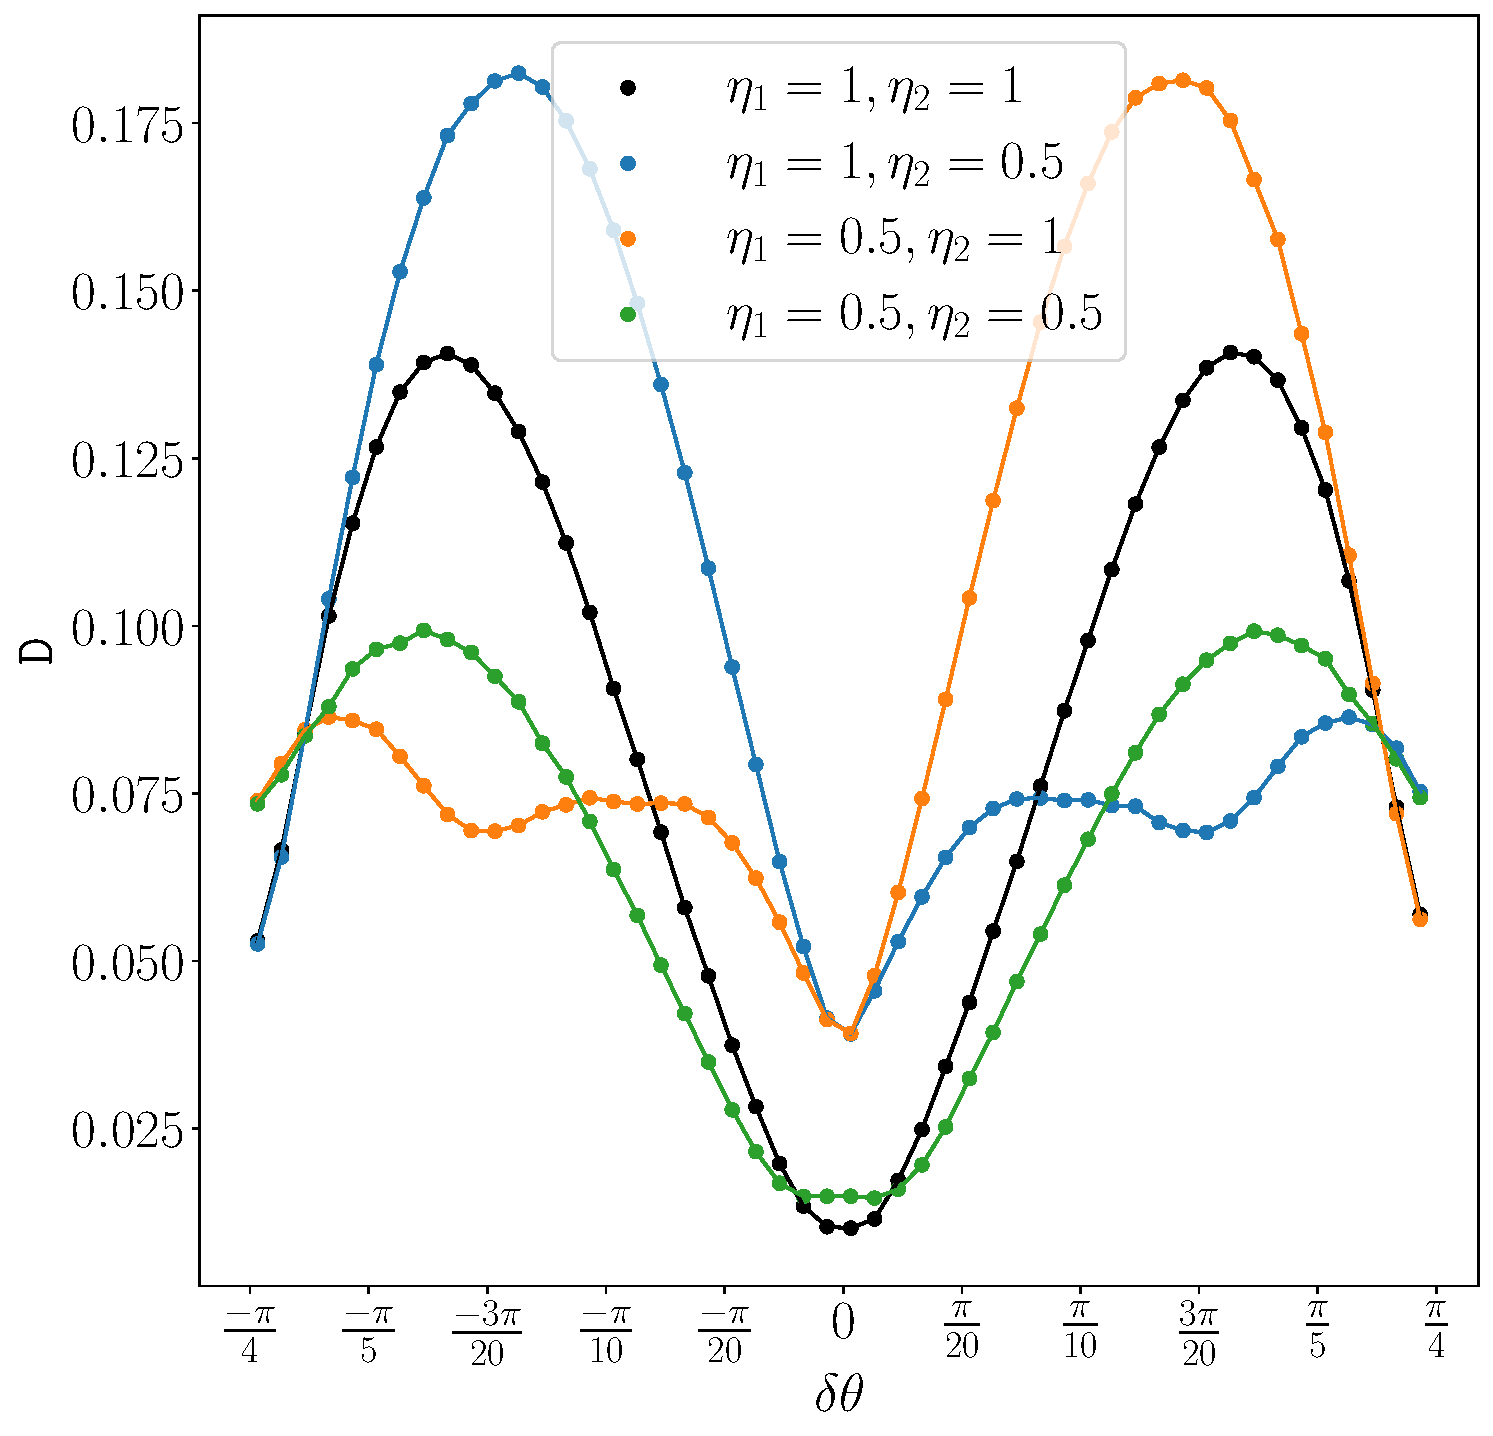
\includegraphics[width=0.75\linewidth]{pics/homodyne/fock.pdf}
    \caption{Numerically calculated distance between the exact distribution of photon count difference in the asymmetrical homodyne scheme and its Gaussian approximation for the single photon signal state as a function of deviation from a balanced beam splitter for different detector efficiencies, with $|\alpha_L|=5$. }%\hl{Note the presence of the same agreement at critical points $\pm\frac{\pi}{4}$ much like the same effect seen at Fig.{~\ref{fig:delta-theta}} -- the same explanation applies here.}}
    \label{fig:fock}
\end{figure}